\documentclass{article}

\usepackage{amsmath}
\usepackage{amssymb}
\usepackage{graphicx}
\usepackage{tikz}
\usetikzlibrary{arrows}
\usepackage{verbatim}
%\usepackage{sfmath}
\usepackage{psfrag}
\usepackage{here} 
\usepackage{hyperref}
\usepackage{xcolor}
\usepackage{tcolorbox}


%\textheight=24cm

%\renewcommand\sfdefault{phv}     %use helvetica for sans serif
\renewcommand{\familydefault}{\sfdefault}
\renewcommand{\familydefault}{cmss}

\begin{document}

\section*{Pr\'actica 3. Tracking and pick-and-place problems for a planar vertical robot manipulator.}

Consider the planar robot manipulator represented in Figure~\ref{fig:figure_1}, which moves in a vertical plane.


\begin{figure}[H]
\centerline{\hspace{0cm}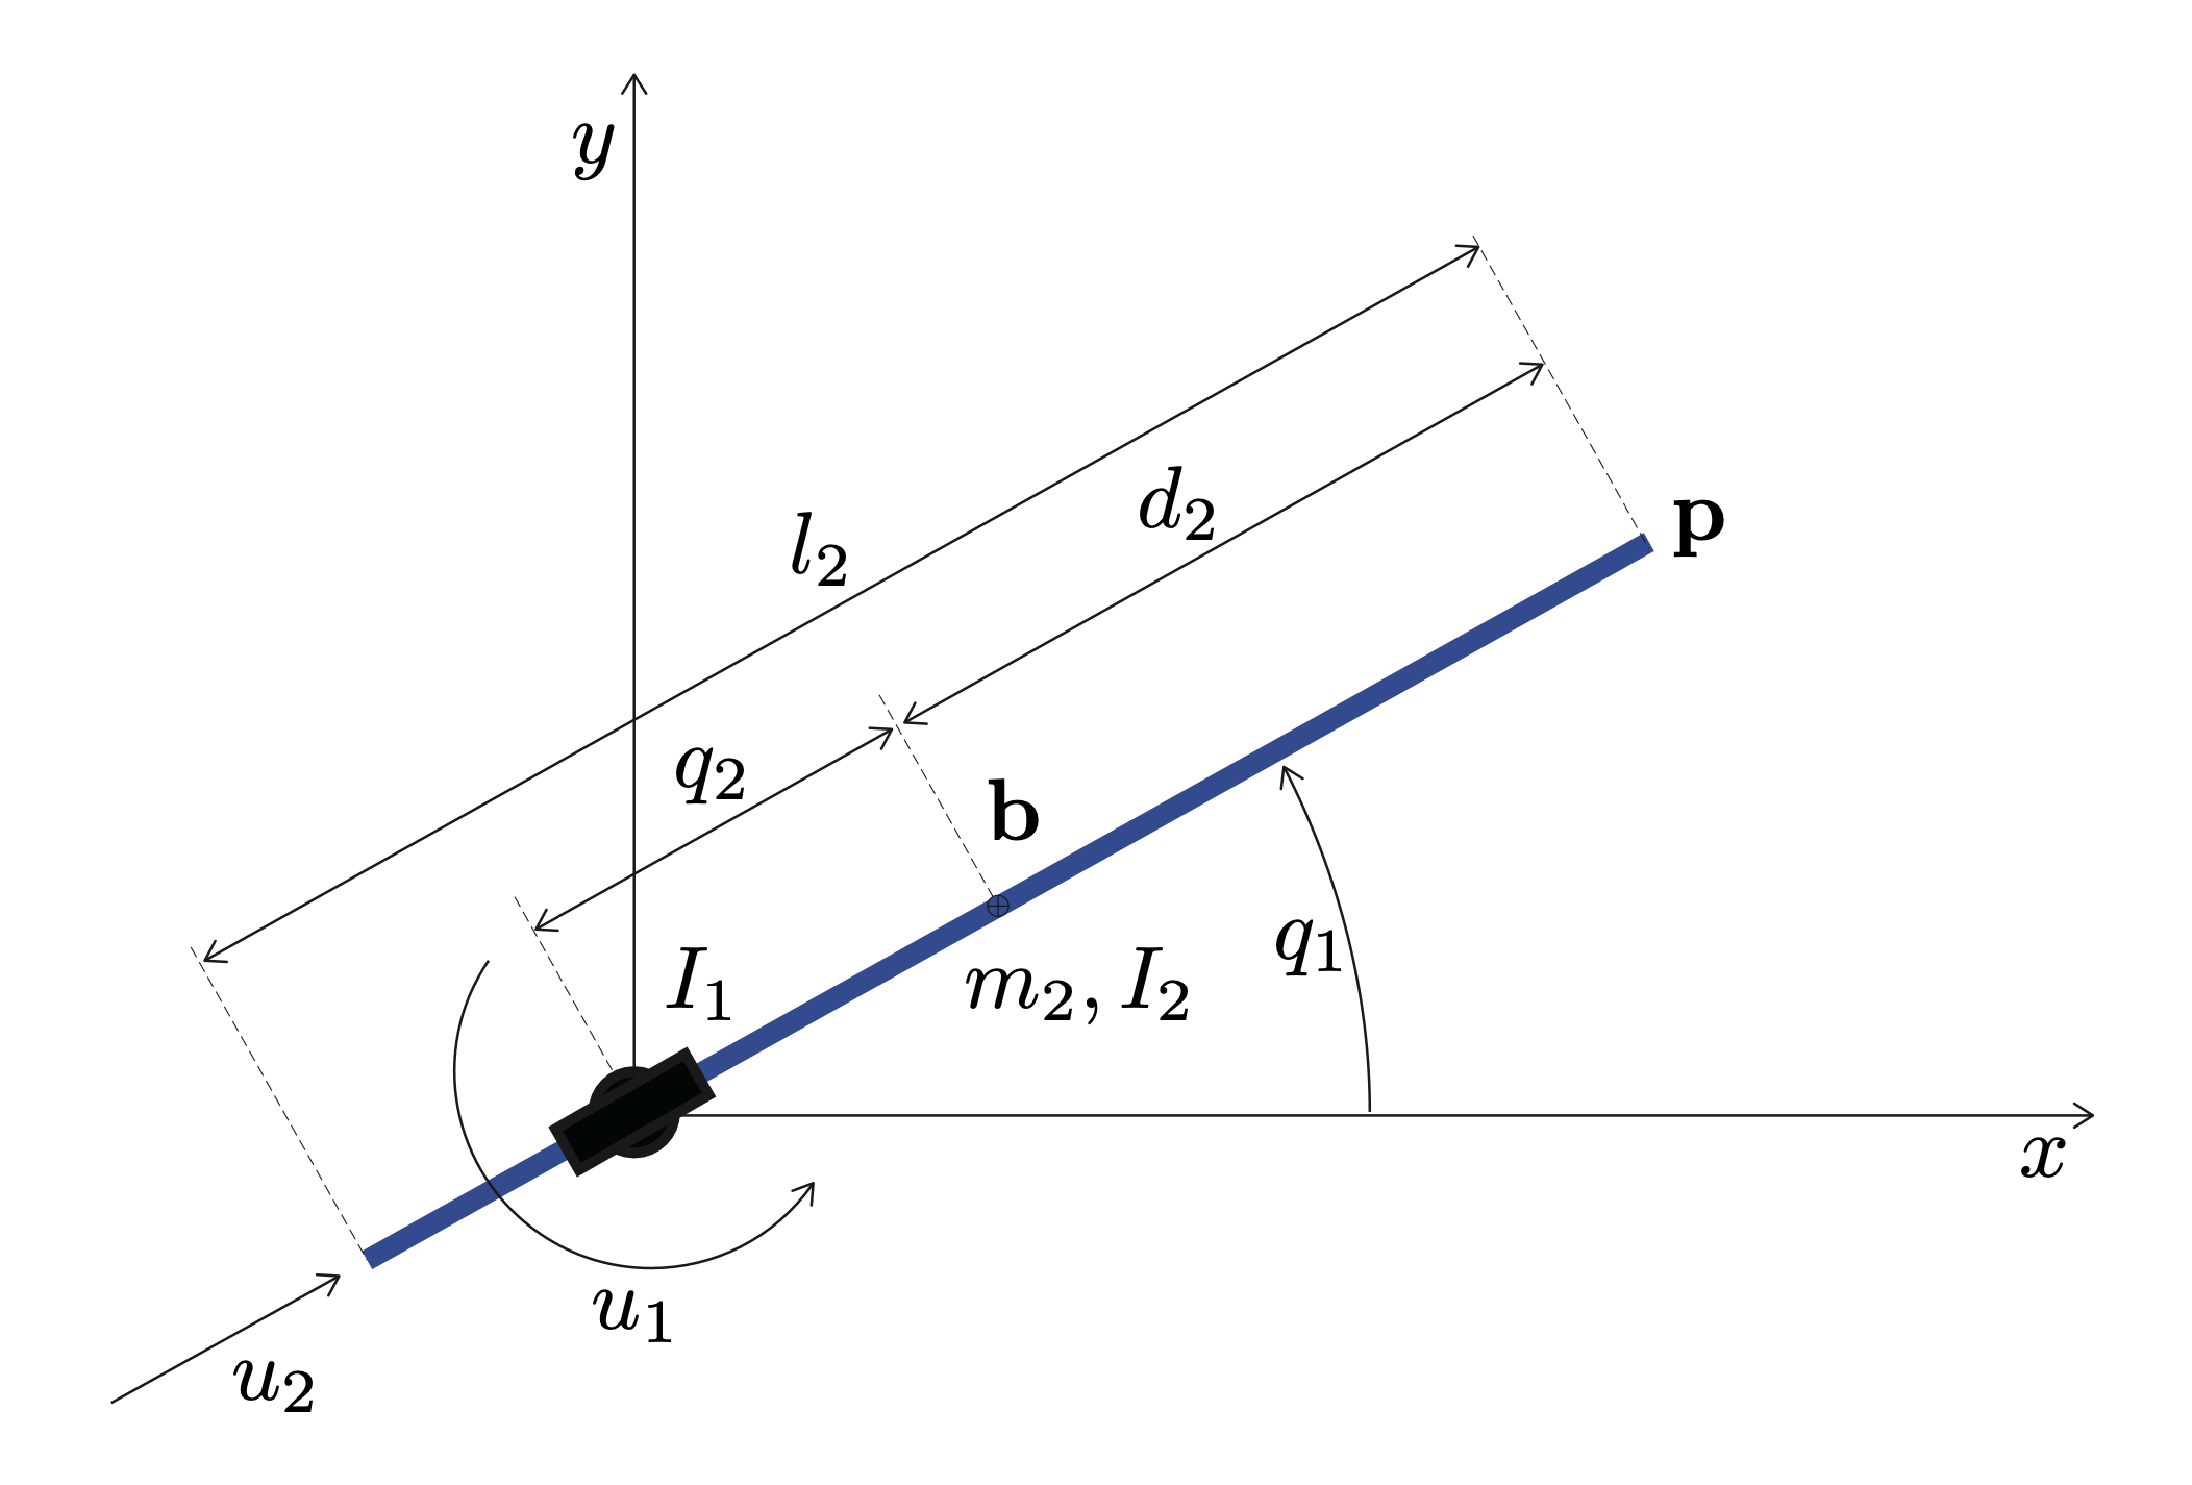
\includegraphics[width=0.66\columnwidth]{figures/drawing.pdf}}
\caption{Planar robot manipulator that moves in a vertical plane.}
\label{fig:figure_1}
\end{figure}


The dynamic model of this robotic system is represented by the
second order differential equation 
\begin{equation*}
\mathbf{B}(\mathbf{q}) \ddot{\mathbf{q}}+ \mathbf{C}(\mathbf{q}, \dot{\mathbf{q}}) + \mathbf{N}(\mathbf{q}) = \mathbf{u},
\end{equation*}
where the two matrices $\mathbf{B}(\mathbf{q})$ and $\mathbf{C}(\mathbf{q}, \dot{\mathbf{q}})$ have the following expressions
\begin{eqnarray*}
\mathbf{B}(\mathbf{q}) &=&
\begin{bmatrix}
I_1 + I_2 + m_2 q_2^2 &0\\
0 & m_2
\end{bmatrix},\\
\mathbf{C}(\mathbf{q}, \dot{\mathbf{q}}) 
&=& 
\begin{bmatrix} 
2 m_2 q_2 \dot{q}_1  \dot{q}_2\\
- m_2 q_2 \dot{q}_1^2
\end{bmatrix},\\
\mathbf{N}(\mathbf{q}) 
&=& 
m_2 g
\begin{bmatrix}
q_2 \cos q_1\\
\sin q_1 
\end{bmatrix}.
\end{eqnarray*}

$
\mathbf{q} =
(
q_1, q_2
)^T
$ 
is the vector of configuration variables, where $q_1$ is the
angular position of the link with respect to the $x$ axis of the reference
frame $\{x, y\}$ and $q_2$ is the linear position of the center of mass $\mathbf{b}$ of the link with respect to the origin of the reference frame.
The
vector
$
\dot{\mathbf{q}} =
(\dot{q}_1,
\dot{q}_2)^T
$ 
is the vector of joint velocities, where $\dot{q}_1$ is an angular
velocity and $\dot{q}_2$ is a linear velovity. The vector
$
\ddot{\mathbf{q}} =
(\ddot{q}_1,
\ddot{q}_2)^T
$
is the vector of accelerations, where  $\ddot{q}_1$ is an angular
acceleration and $\ddot{q}_2$ is a linear acceleration. The control inputs of the system are
$
\mathbf{u} =
(u_1,
u_2)^T
$,
where $u_1$ is the torque applied by the angular actuator to the link and
$u_2$ is the force applied by the linear actuator to the link. 
$I_1$ is the barycentric moment of inertia of the angular and linear actuators,
$I_2$ is the barycentric moment of inertia of the link, and $m_2$ is the mass of the link.

\newpage

Consider the following two robotic tasks.

\begin{itemize}

\item[1)]
Tracking task:  follow with the tip $\mathbf{p}$ a setpoint describing a circle centred at $(0.5, 0.5)$ m with radius $0.25$ m which moves clockwise with angular velocity $0.25$ rad/s. 

\item[2)]
Pick and place task: move iteratively the tip $\mathbf{p}$ between the setpoints $\mathbf{p}_A = (-0.5, 0.75)$ m and 
$\mathbf{p}_B = (0.5, 0.25)$ m. The motions must be rest to rest.

\end{itemize}

Assume that the initial state of the manipulator is $(q_1, q_2, \dot{q}_1, \dot{q}_2)^T= (0, 0, 0, 0)^T$. 
Assume that 
$I_1=1$ kg m$^2$,
$I_2=1$  kg m$^2$,
$m_2=1$ kg,
$l_2=1$ m,
$d_2=0.5$ m,
$g=9.81$ m/s$^2$.




\begin{itemize}
\item[a.] Demonstrate the equations of the dynamic model using the Lagrange method. (Copia la soluci\'on del la Pr\'actica 1)



\item[b.] 
Compute the state space representation of the dynamics of the manipulator in which $\mathbf{x} = (x_1,x_2,x_3,x_4)^T= (q_1, q_2, \dot{q}_1, \dot{q}_2)^T$. Take the coordinates of point $\mathbf{p}$ as output variables. (Copia la soluci\'on del la Pr\'actica 1)
 
\item[c.]
Compute the relation between the configuration variables 
$\mathbf{q} =(q_1, q_2)^T$ 
and the position of the tip $\mathbf{p} = (p_1, p_2)^T$.
(Copia la soluci\'on del la Pr\'actica 1)

\item[d.]
Compute the Jacobian matrix of the relation determined in c. (Contesta en el informe y sube el c\'odigo \texttt{Matlab} a Aula Virtual en el fichero \texttt{j\_manipulator.m})

\item[e.] 
Compute the time derivative of the Jacobian matrix determined in d. (Contesta en el informe y sube el c\'odigo \texttt{Matlab} a Aula Virtual en el fichero \texttt{dot\_j\_manipulator.m})



\item[f.]  Design a controller based on the transpose Jacobian method to execute the tracking task. Write a \texttt{Matlab} code that implements the controller to execute the task. Show, plotting the relevant variables and an animation, that the controller satisfies the specifications. (Contesta en el informe y sube el c\'odigo \texttt{Matlab} a Aula Virtual en la carpeta \texttt{controller\_jt})


\item[g.] Design a controller based on the feedback linearization method to execute the pick and place task. Write a \texttt{Matlab} code that implements the controller to execute the task. Show, plotting the relevant variables and an animation, that the controller satisfies the specifications. (Contesta en el informe y sube el c\'odigo \texttt{Matlab} a Aula Virtual en la carpeta \texttt{controller\_fl})


\end{itemize}



\noindent
\textcolor{red}{Write a detailed report answering each question in a different section. Explain each result obtained and motivate each choice made during the design process. Include the \texttt{Matlab} code in the corresponding section in the written report. Additionally, upload the \texttt{Matlab} code of each section of the project in a separate folder. Originality and completeness of the answers will be the aspects that will be taken into account in the grading of the project, and therefore, the \texttt{Matlab} code alone will not be considered.} 


\newpage













\section*{Solution of Pr\'actica 3}


\begin{itemize}

\item[a.] 
{\color{gray}
Demonstrate the equations of the dynamic model using the Lagrange method. (Copia la soluci\'on del la Pr\'actica 1)
}

\bigskip

Mediante el metodo de Lagrange hallamos las ecuaciones de estado del modelo dinamico, sabiendo que: L = T - V\\

La energía cinética T se descompone en la suma de la energía cinética angular y lineal:\\\\
$T_{ang} = \frac{1}{2}(I_1 + I_2)\dot{q_1}^2$,\\\\

$T_{lin} = \frac{1}{2}m_2\dot{q_1}^2q_2^2 + \frac{1}{2}m_2\dot{q_2}^2$\\

La energía potencial es $V = m_2gh$, siendo $h = q_2_y = sen(q_1)q_2$.

Por tanto,\\

$L = \frac{1}{2}(I_1 + I_2 + m_2q_2^2)\dot{q_1}^2 + \frac{1}{2}m_2\dot{q_2}^2 - m_2gsen(q_1)q_2$\\

De este modo, obtenemos las dos siguientes ecuaciones de Lagrange,\\
la primera:\\

		$\frac{\partial L}{\partial \dot{q_1}} = (I_1 + I_2)\dot{q_1} + m_2q_2^2\dot{q_1}$\\\\
		$\frac{d}{dt}\frac{\partial L}{\partial \dot{q_1}} = (I_1 + I_2 + m_2q_2^2)\ddot{q_1} + 2mq_1\dot{q_1}\dot{q_2}$\\\\
		$\frac{\partial L}{\partial q_1} = -m_2gcos(q_1)q_2$\\\\
		
		$(I_1 + I_2 + m_2q_2^2)\ddot{q_1} + 2mq_2\dot{q_1}\dot{q_2} + m_2gcos(q_1)q_2 = u_1$\\
		
y la segunda:\\\\
		$\frac{\partial L}{\partial \dot{q_2}} = m_2\dot{q_2}$\\\\
		$\frac{d}{dt}\frac{\partial L}{\partial \dot{q_2}} = m_2\ddot{q_2}$\\\\
		$\frac{\partial L}{\partial q_2} = m_2q_2\dot{q_1}^2 - m_2gsen(q_1)$\\\\
		
		$m_2\ddot{q_2} - m_2q_2\dot{q_1}^2 + m_2gsen(q_1) = u_2$\\
		

Por lo tanto, escribiendo las ecuaciones en forma matricial obtenemos:\\

$\begin{bmatrix}
I_1 + I_2 + m_2 q_2^2 &0\\
0 & m_2
\end{bmatrix}\ddot{q}
 + 
\begin{bmatrix} 
2 m_2 q_2 \dot{q}_1  \dot{q}_2\\
- m_2 q_2 \dot{q}_1^2
\end{bmatrix}
 + 
\begin{bmatrix}
m_2gcos(q_1)q_2\\
m_2gsen(q_1)
\end{bmatrix}
 = u
$

Finalmente,

	$\ddot{q} = \begin{pmatrix}
	\frac{2\dot{q_1}\dot{q_2}m_2q_2 - u_1 + gm_2q_2cos(q_1))}{m_2q_2^2 + I_1 + I_2}\\
	\frac{m_2q_2\dot{q_1}^2 + u_2 - gm_2sin(q_1)}{m_2}
	\end{pmatrix}
	$
		


\bigskip










\item[b.] 
{\color{gray}
Compute the state space representation of the dynamics of the manipulator in which $\mathbf{x} = (x_1,x_2,x_3,x_4)^T= (q_1, q_2, \dot{q}_1, \dot{q}_2)^T$. Take the coordinates of point $\mathbf{p}$ as output variables. (Copia la soluci\'on del la Pr\'actica 1)
 }
 
 \bigskip
Asumiendo que:\\\\
		$x = 
			\begin{pmatrix}
				 x_1\\x_2\\x_3\\x_4
			\end{pmatrix}
		 		= 
			\begin{pmatrix}
				 q_1\\q_2\\\dot{q_1}\\\dot{q_2}
			\end{pmatrix}$,\\\\
podemos escribir:\\\\
		$\frac{d}{dt}
			\begin{pmatrix}
				 q_1\\q_2\\\dot{q_1}\\\dot{q_2}
			\end{pmatrix}
				=
			\begin{pmatrix}
				 \dot{q_1}\\\dot{q_2}\\\ddot{q_1}\\\ddot{q_2}
			\end{pmatrix}
				=
			\begin{pmatrix}
				 \dot{q_1}\\\dot{q_2}\\\frac{2\dot{q_1}\dot{q_2}m_2q_2 - u_1 + gm_2q_2cos(q_1))}{m_2q_2^2 + I_1 + I_2}\\\frac{m_2q_2\dot{q_1}^2 + u_2 - gm_2sin(q_1)}{m_2}
			\end{pmatrix}$.\\\\
Por tanto, la representacion del espacio de estados es:

	$\dot{x_1}=x_3$,\\
	$\dot{x_2}=x_4$,\\
	$\dot{x_3}=\frac{2\dot{q_1}\dot{q_2}m_2q_2 - u_1 + gm_2q_2cos(q_1))}{m_2q_2^2 + I_1 + I_2}$,\\
	$\dot{x_4}=\frac{m_2q_2\dot{q_1}^2 + u_2 - gm_2sin(q_1)}{m_2}$.\\
	
Tomando las coordenadas del punto P como outputs obtenemos:

$P_x = cos(q_1)(q_2+d_2)$\\
$P_y = sen(q_1)(q_2+d_2)$.
\bigskip
 
 
 
 
 
 
 
 
 
 
 
\item[c.]
{\color{gray}
Compute the relation between the configuration variables 
$\mathbf{q} =(q_1, q_2)^T$ 
and the position of the tip $\mathbf{p} = (p_1, p_2)^T$.
(Copia la soluci\'on del la Pr\'actica 1)
}

\bigskip
La relacion entre las variables de configuracion $\mathbf{q} =(q_1, q_2)^T$ y la posicion del pico $\mathbf{p} = (p_1, p_2)^T$ es:\\
$P_x = cos(q_1)(q_2+d_2)$\\
$P_y = sen(q_1)(q_2+d_2)$.
\bigskip










\item[d.]
{\color{gray}
Compute the Jacobian matrix of the relation determined in c. (Contesta en el informe y sube el c\'odigo \texttt{Matlab} a Aula Virtual en el fichero \texttt{j\_manipulator.m})
}

\bigskip
La matriz Jacobiana de la relacion determinada en el apartado anterior se halla mediante el siguiente codigo de matlab:
\bigskip


\begin{tcolorbox}
[
%width=12cm,
title={File \texttt{j\_manipulator.m}}      
]
\begin{scriptsize}
\begin{verbatim}

clear all
close all
clc

syms d2 q1 q2

Px = cos(q1)*(q2 + d2);
Py = sin(q1)*(q2 + d2);


J = jacobian([Px, Py], [q1, q2])

\end{verbatim}
\end{scriptsize}
\end{tcolorbox}

Obteniendo la siguiente matriz:\\
$J =

\begin{equation}
\begin{bmatrix}
-sin(q1)*(d2 + q2) & cos(q1)\\
cos(q1)*(d2 + q2) & sin(q1)
\end{bmatrix}
\end{equation}$







\item[e.] 
{\color{gray}
Compute the time derivative of the Jacobian matrix determined in d. (Contesta en el informe y sube el c\'odigo \texttt{Matlab} a Aula Virtual en el fichero \texttt{dot\_j\_manipulator.m})
}

\bigskip
La matriz Jacobiana en funcion de la derivada del tiempo a partir de la matriz hallada en el apartado anterior se halla con el siguiente codigo de matlab:
\bigskip


\begin{tcolorbox}
[
%width=12cm,
title={File \texttt{dot\_j\_manipulator.m}}      
]
\begin{scriptsize}
\begin{verbatim}

clear all
close all
clc

syms d1 d2 x1(t) x2(t)

J = [-sin(x1(t))*(d2 + x2(t)), cos(x1(t));
    cos(x1(t))*(d2 + x2(t)), sin(x1(t))];

Jdot = diff(J,t)

\end{verbatim}
\end{scriptsize}
\end{tcolorbox}


Obteniendo la siguiente matriz:\\

$\dot{J} =

\begin{equation}
\begin{bmatrix}
-sin(x1(t))*diff(x2(t), t) - cos(x1(t))*(d2 + x2(t))*diff(x1(t), t), -sin(x1(t))*diff(x1(t), t)\\
cos(x1(t))*diff(x2(t), t) - sin(x1(t))*(d2 + x2(t))*diff(x1(t), t),  cos(x1(t))*diff(x1(t), t)
\end{bmatrix}
\end{equation}$












\item[f.]  
{\color{gray}
Design a controller based on the transpose Jacobian method to execute the tracking task. Write a \texttt{Matlab} code that implements the controller to execute the task. Show, plotting the relevant variables and an animation, that the controller satisfies the specifications. (Contesta en el informe y sube el c\'odigo \texttt{Matlab} a Aula Virtual en la carpeta \texttt{controller\_jt})
}


\bigskip
A partir de los datos obtenidos en los anteriores apartados, podemos diseñar un controlador a partir del metodo de la matriz jacobiana traspuesta para ejecutar la tarea de seguimiento.
Los valores de Kp y Kd han sido escogidos a base de ensayo y error.
\bigskip


\begin{tcolorbox}
[
%width=12cm,
title={File \texttt{controller\_jt\_init.m}}   
]
\begin{scriptsize}
\begin{verbatim}

close all; 
clear all; 
clc;


figure
grid
hold

xmin=0;
xmax=25;
ymin=-1.5;
ymax=2;

axis([xmin xmax ymin ymax]); 
axis ('square');

\end{verbatim}
\end{scriptsize}
\end{tcolorbox}

\begin{tcolorbox}
[
%width=12cm,
title={File \texttt{controller\_jt\_f.m}}      
]
\begin{scriptsize}
\begin{verbatim}

function  xdot  = controller_jt_f(x,u)

x1 = x(1);
x2 = x(2);
x3 = x(3);
x4 = x(4);

u1 = u(1);
u2 = u(2);

I1 = 1;
I2 = 1;
m2 = 1;
g = 9.81;

B = [I1 + I2 + m2*x2^2, 0;
     0, m2];

C = [2*m2*x2*x3*x4;
    -m2*x2*x3^2];

N = m2*g*[x2*cos(x1);
          sin(x1)];

invB = inv(B);

v = -invB*C - invB*N + invB*[u1;u2];

xdot = [x3;x4;v(1);v(2)];

end

\end{verbatim}
\end{scriptsize}
\end{tcolorbox}

\begin{tcolorbox}
[
%width=12cm,
title={File \texttt{draw\_circle.m}}      
]
\begin{scriptsize}
\begin{verbatim}

function draw_circle(xcenter,ycenter,radius)
    angle = 0:pi/50:2*pi;
    xcircle = radius * cos(angle) + xcenter;
    ycircle = radius * sin(angle) + ycenter;
    h = plot(xcircle, ycircle,'b','LineWidth',0.1);
end

\end{verbatim}
\end{scriptsize}
\end{tcolorbox}


\begin{tcolorbox}
[
%width=12cm,
title={File \texttt{controller\_jt\_draw.m}}      
]
\begin{scriptsize}
\begin{verbatim}

function controller_jt_draw(x)

    l2=1;

    xtip = l2*cos(x(1,:))*(x(2,:) + 0.5);
    ytip = l2*sin(x(1,:))*(x(2,:) + 0.5);

    axis([-0.5 1.5 -0.5 1.5])

    hold on;

    axis square

    draw_circle(0.5,0.5,0.25);

    %plot([0,0], [0,0],'r','LineWidth',0.1)
    plot([0,xtip], [0,ytip],'r','LineWidth',0.1)
 

 drawnow;

\end{verbatim}
\end{scriptsize}
\end{tcolorbox}


\begin{tcolorbox}
[
%width=12cm,
title={File \texttt{controller\_jt\_main.m}}      
]
\begin{scriptsize}
\begin{verbatim}

clear all
close all
clc

init;

x = [0; 0; 0; 0]; % Estado inicial
u = [0; 0];

dt=0.01;

frame_counter=0;
 
Kp = [70, 0;
      0, 90];

Kd = [8, 0;
      0, 16];

I1 = 1;
I2 = 1;
m2 = 1;
d2 = 0.5;
l2 = 1;
r = 0.25;
g = 9.81;

for t=0:dt:30

    x1 = x(1);
    x2 = x(2);
    x3 = x(3);
    x4 = x(4);

    px = l2*cos(x1)*(x2 + d2);
    py = l2*sin(x1)*(x2 + d2);
    
    p = [px;py];

    pd = [0.5;0.5] + r*[cos(0.25*t);sin(0.25*t)];
    dotpd = r*[-sin(0.25*t);cos(0.25*t)];
    ddotpd = r*[-cos(0.25*t);-sin(0.25*t)];

    % Jacobian
    J = [-sin(x1)*(d2 + x2), cos(x1);
        cos(x1)*(d2 + x2), sin(x1)];

    Jdot = [-sin(x1)*x4 - cos(x1)*(d2 + x2)*x3, -sin(x1)*x3;
            cos(x1)*x4 - sin(x1)*(d2 + x2)*x3, cos(x1)*x4];

    N = m2*g*[x2*cos(x1);
              sin(x1)];

    B = [I1+I2+m2*x2^2, 0;
        0, m2];

    C = [2*m2*x2*x3*x4;
        -m2*x2*x3^2];

    v = inv(J)*(ddotpd + Kd*(dotpd-J*[x3;x4]) + Kp*(pd-p) - Jdot*[x3;x4]);
    
    u = B*v+C+N;

    x = x + controller_jt_f(x,u)*dt; % Euler
    %x=x+dt*(0.25*controller_jt_f(x,u)+0.75*
    	%(controller_jt_f(x+dt*(2/3)*controller_jt_f(x,u),u))); % Runge-Kutta
    
    frame_counter = frame_counter+1;
    pause(dt);

    % Frame sampling
    if frame_counter == 10
        %plot(t,x(1),'k--.',t,x(2),'r--.',t,u(1),'g--.', t,u(2),'b--.');
        controller_jt_draw(x);
        frame_counter =0;
    end
end 

\end{verbatim}
\end{scriptsize}
\end{tcolorbox}




\begin{figure}[H]
\centerline{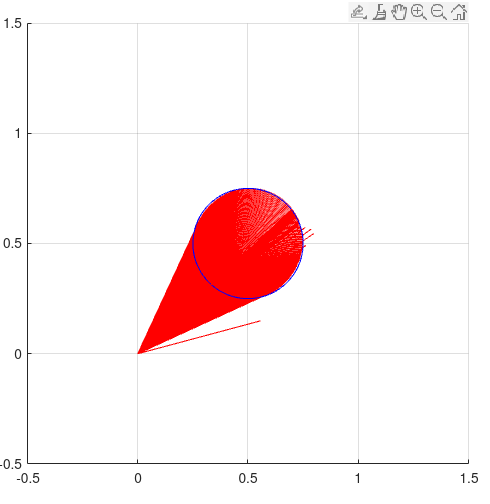
\includegraphics[width=0.75\columnwidth]{figures/controller_jt}}
\caption{controller\_jt}
\label{fig:figure_2}
\end{figure}

















\item[g.] 
{\color{gray}
Design a controller based on the feedback linearization method to execute the pick and place task. Write a \texttt{Matlab} code that implements the controller to execute the task. Show, plotting the relevant variables and an animation, that the controller satisfies the specifications. (Contesta en el informe y sube el c\'odigo \texttt{Matlab} a Aula Virtual en la carpeta \texttt{controller\_fl})
}

\bigskip
En este caso, diseñaremos un controlador basado en el metodo de linealizacion de retroalimentacion para ejecutar la tarea de recoger y colocar. Al igual que en el apartado anterior, los valores de Kp y Kd han sido escogidos a base de ensayo y error.
\bigskip


\begin{tcolorbox}
[
%width=12cm,
title={File \texttt{controller\_fl\_init.m}}   
]
\begin{scriptsize}
\begin{verbatim}

close all; 
clear all; 
clc;

figure
grid
hold

xmin=0;
xmax=25;
ymin=-1.5;
ymax=2;

axis([xmin xmax ymin ymax]); 
axis ('square');

\end{verbatim}
\end{scriptsize}
\end{tcolorbox}

\begin{tcolorbox}
[
%width=12cm,
title={File \texttt{controller\_fl\_f.m}}      
]
\begin{scriptsize}
\begin{verbatim}

function  xdot  = controller_fl_f(x,u)

x1 = x(1);
x2 = x(2);
x3 = x(3);
x4 = x(4);

u1 = u(1);
u2 = u(2);

I1 = 1;
I2 = 1;
m2 = 1;
g = 9.81;

B = [I1 + I2 + m2*x2^2, 0;
     0, m2];

C = [2*m2*x2*x3*x4;
    -m2*x2*x3^2];

N = m2*g*[x2*cos(x1);
          sin(x1)];

invB = inv(B);

v = -invB*C - invB*N + invB*[u1;u2];

 
xdot = [x3;x4;v(1);v(2)];

end


\end{verbatim}
\end{scriptsize}
\end{tcolorbox}

\begin{tcolorbox}
[
%width=12cm,
title={File \texttt{controller\_fl\_draw.m}}      
]
\begin{scriptsize}
\begin{verbatim}

function controller_fl_draw(x)

    l2=1;

    xtip = l2*cos(x(1,:))*(x(2,:) + 0.5);
    ytip = l2*sin(x(1,:))*(x(2,:) + 0.5);

    axis([-1 1 -1 2])

    hold on;

    axis square

    plot([0,xtip], [0,ytip],'r','LineWidth',0.1)
 

 drawnow;

\end{verbatim}
\end{scriptsize}
\end{tcolorbox}


\begin{tcolorbox}
[
%width=12cm,
title={File \texttt{controller\_fl\_main.m}}      
]
\begin{scriptsize}
\begin{verbatim}

clear all
close all
clc

init;

x = [0; 0; 0; 0]; % Estado inicial
u = [0; 0];

pdA = [-0.5;0.75];
pdB = [0.5;0.25];

dt=0.01;

frame_counter=0;

Kp = [80, 0;
      0, 100];

Kd = [16, 0;
      0, 32];

I1 = 1;
I2 = 1;
m2 = 1;
d2 = 0.5;
l2 = 1;
r = 0.25;
g = 9.81;

for t=0:dt:10

    x1 = x(1);
    x2 = x(2);
    x3 = x(3);
    x4 = x(4);

    px = l2*cos(x1)*(x2 + d2);
    py = l2*sin(x1)*(x2 + d2);
    
    p = [px;py];

    gl = square(0.66*t);
    
    % Jacobian
    J = [-sin(x1)*(d2 + x2), cos(x1);
        cos(x1)*(d2 + x2), sin(x1)];

    Jdot = [-sin(x1)*x4 - cos(x1)*(d2 + x2)*x3, -sin(x1)*x3;
            cos(x1)*x4 - sin(x1)*(d2 + x2)*x3, cos(x1)*x4];

    if gl == 1
        u = J'*Kp*(pdA - p) - J'*Kd*J*[x3;x4];
    else
        u = J'*Kp*(pdB - p) - J'*Kd*J*[x3;x4];
    end

    x = x + controller_fl_f(x,u)*dt; % Euler
    %x=x+dt*(0.25*controller_fl_f(x,u)+0.75*
    	%(controller_fl_f(x+dt*(2/3)*controller_fl_f(x,u),u))); % Runge-Kutta

    
    frame_counter = frame_counter+1;
    pause(dt);

    % Frame sampling
    if frame_counter == 10
        %plot(t,x(1),'k--.',t,x(2),'r--.',t,u(1),'g--.', t,u(2),'b--.');
        controller_fl_draw(x);
        frame_counter =0;
    end
end

\end{verbatim}
\end{scriptsize}
\end{tcolorbox}



\begin{figure}[H]	
\centerline{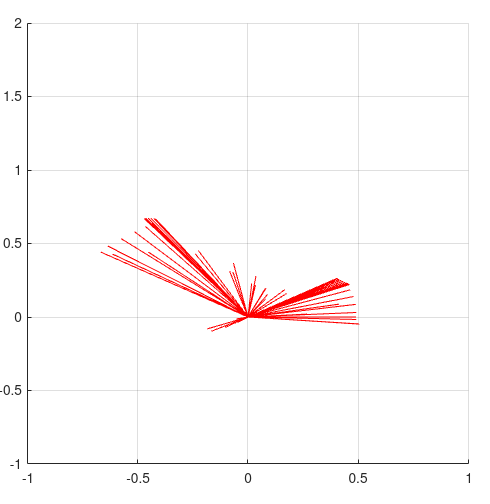
\includegraphics[width=0.75\columnwidth]{figures/controller_fl}}
\caption{controller\_fl.}
\label{fig:figure_4}
\end{figure}


\end{itemize}





















\end{document}
